\FloatBarrier
\subsubsection{Przykład}
\begin{figure}[h]
	\centering
	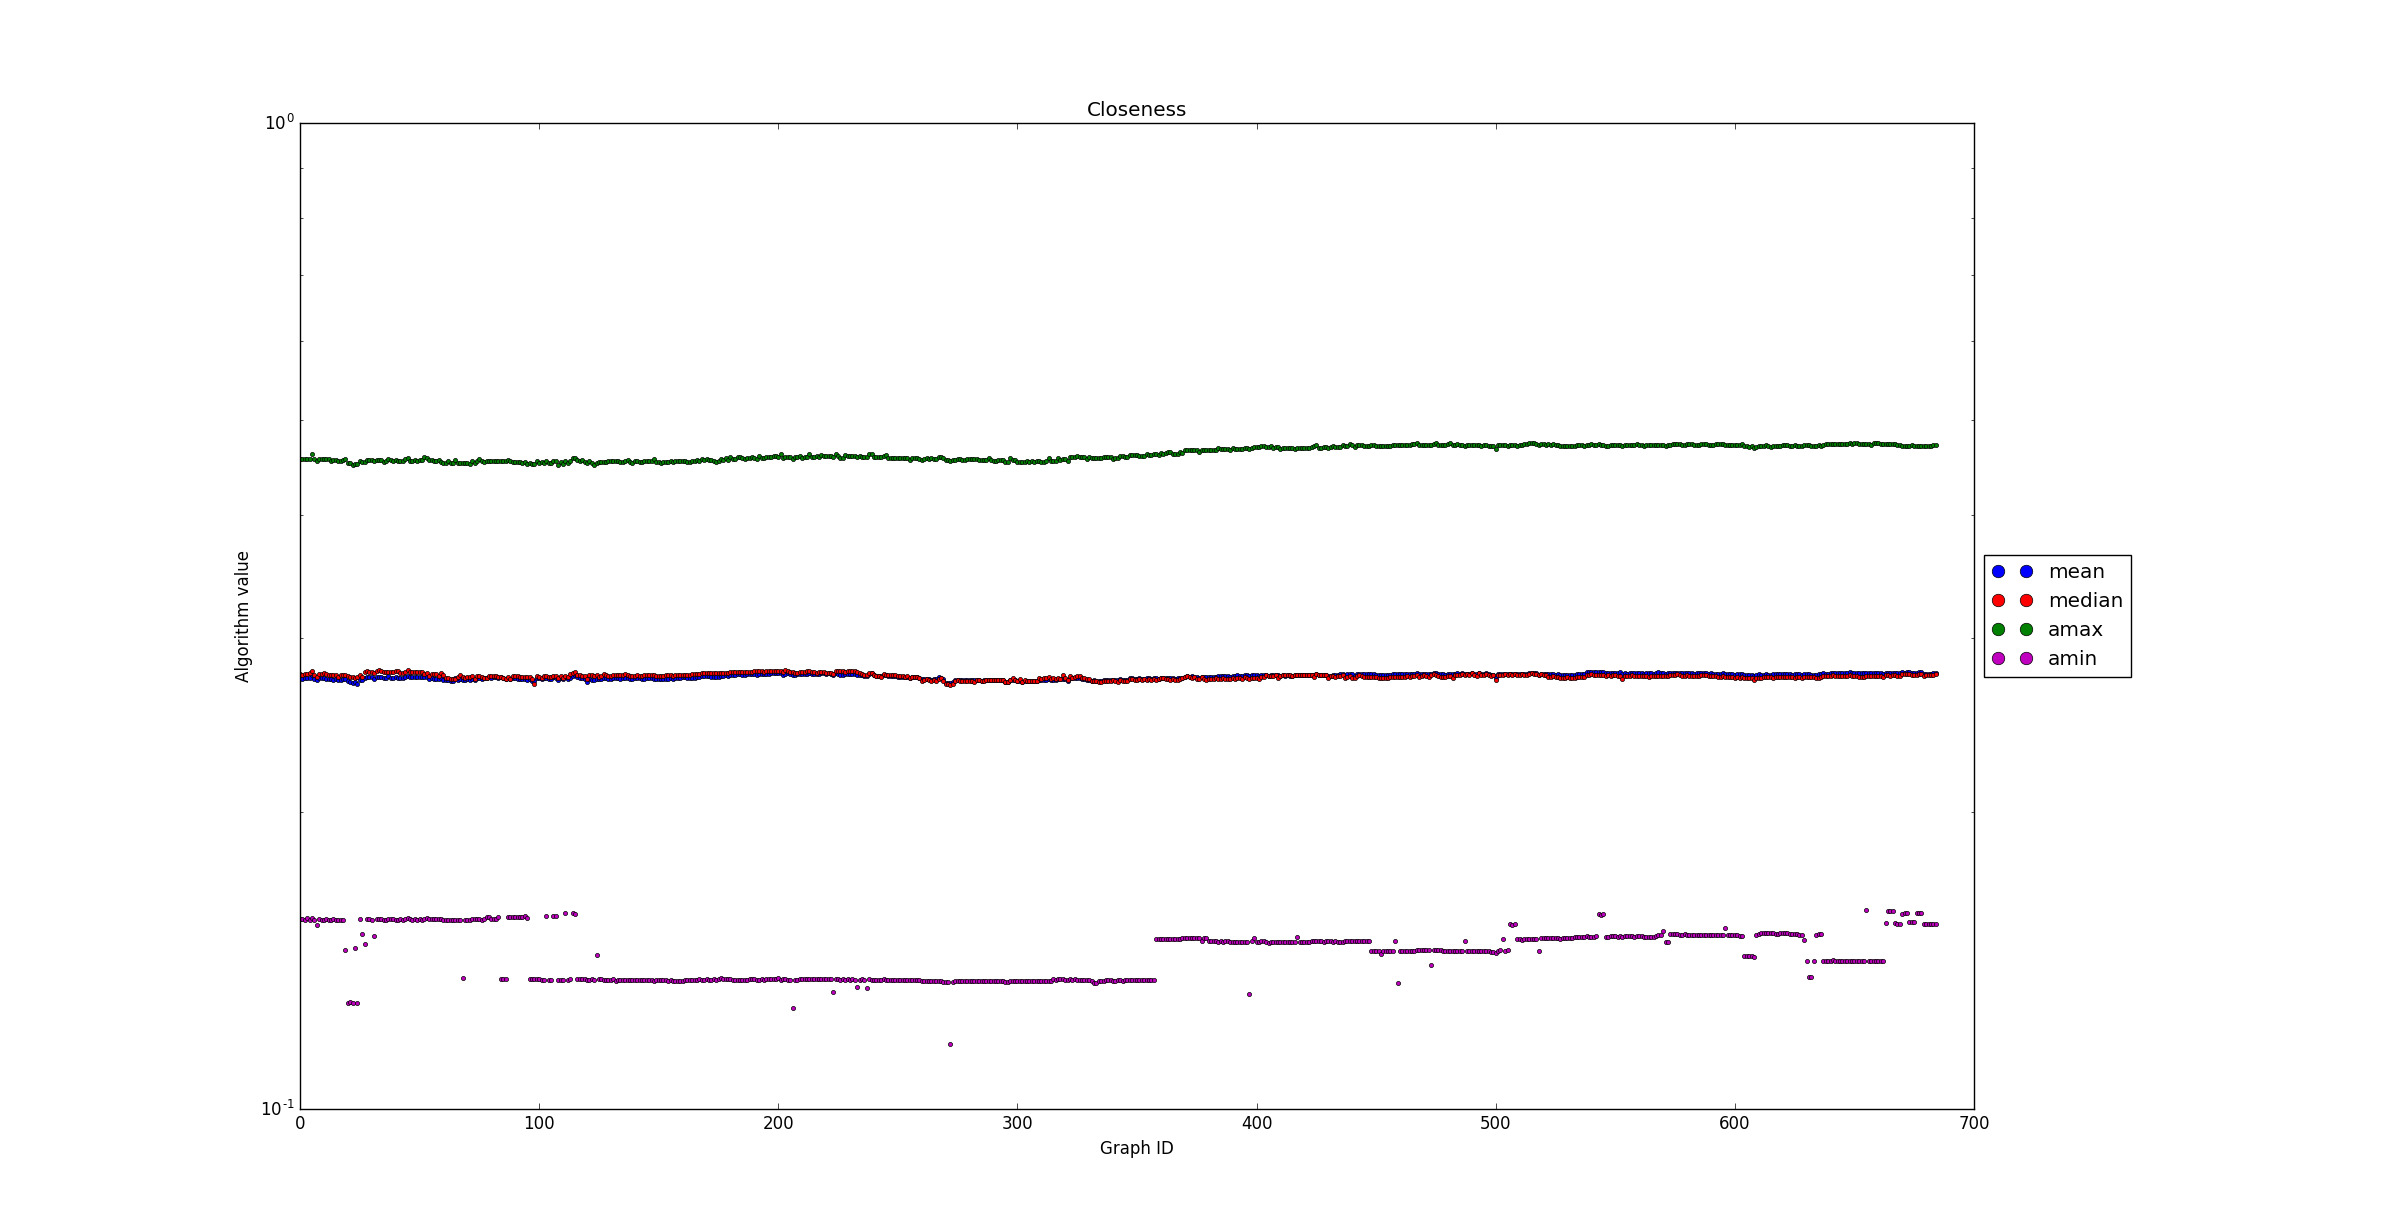
\includegraphics[width=\textwidth]{closeness}
	\caption{Działanie Betweenness Centrality  na przykładowym grafie}
\end{figure}
\FloatBarrier\FloatBarrier
\subsubsection{Przykład}
\begin{figure}[h]
	\centering
	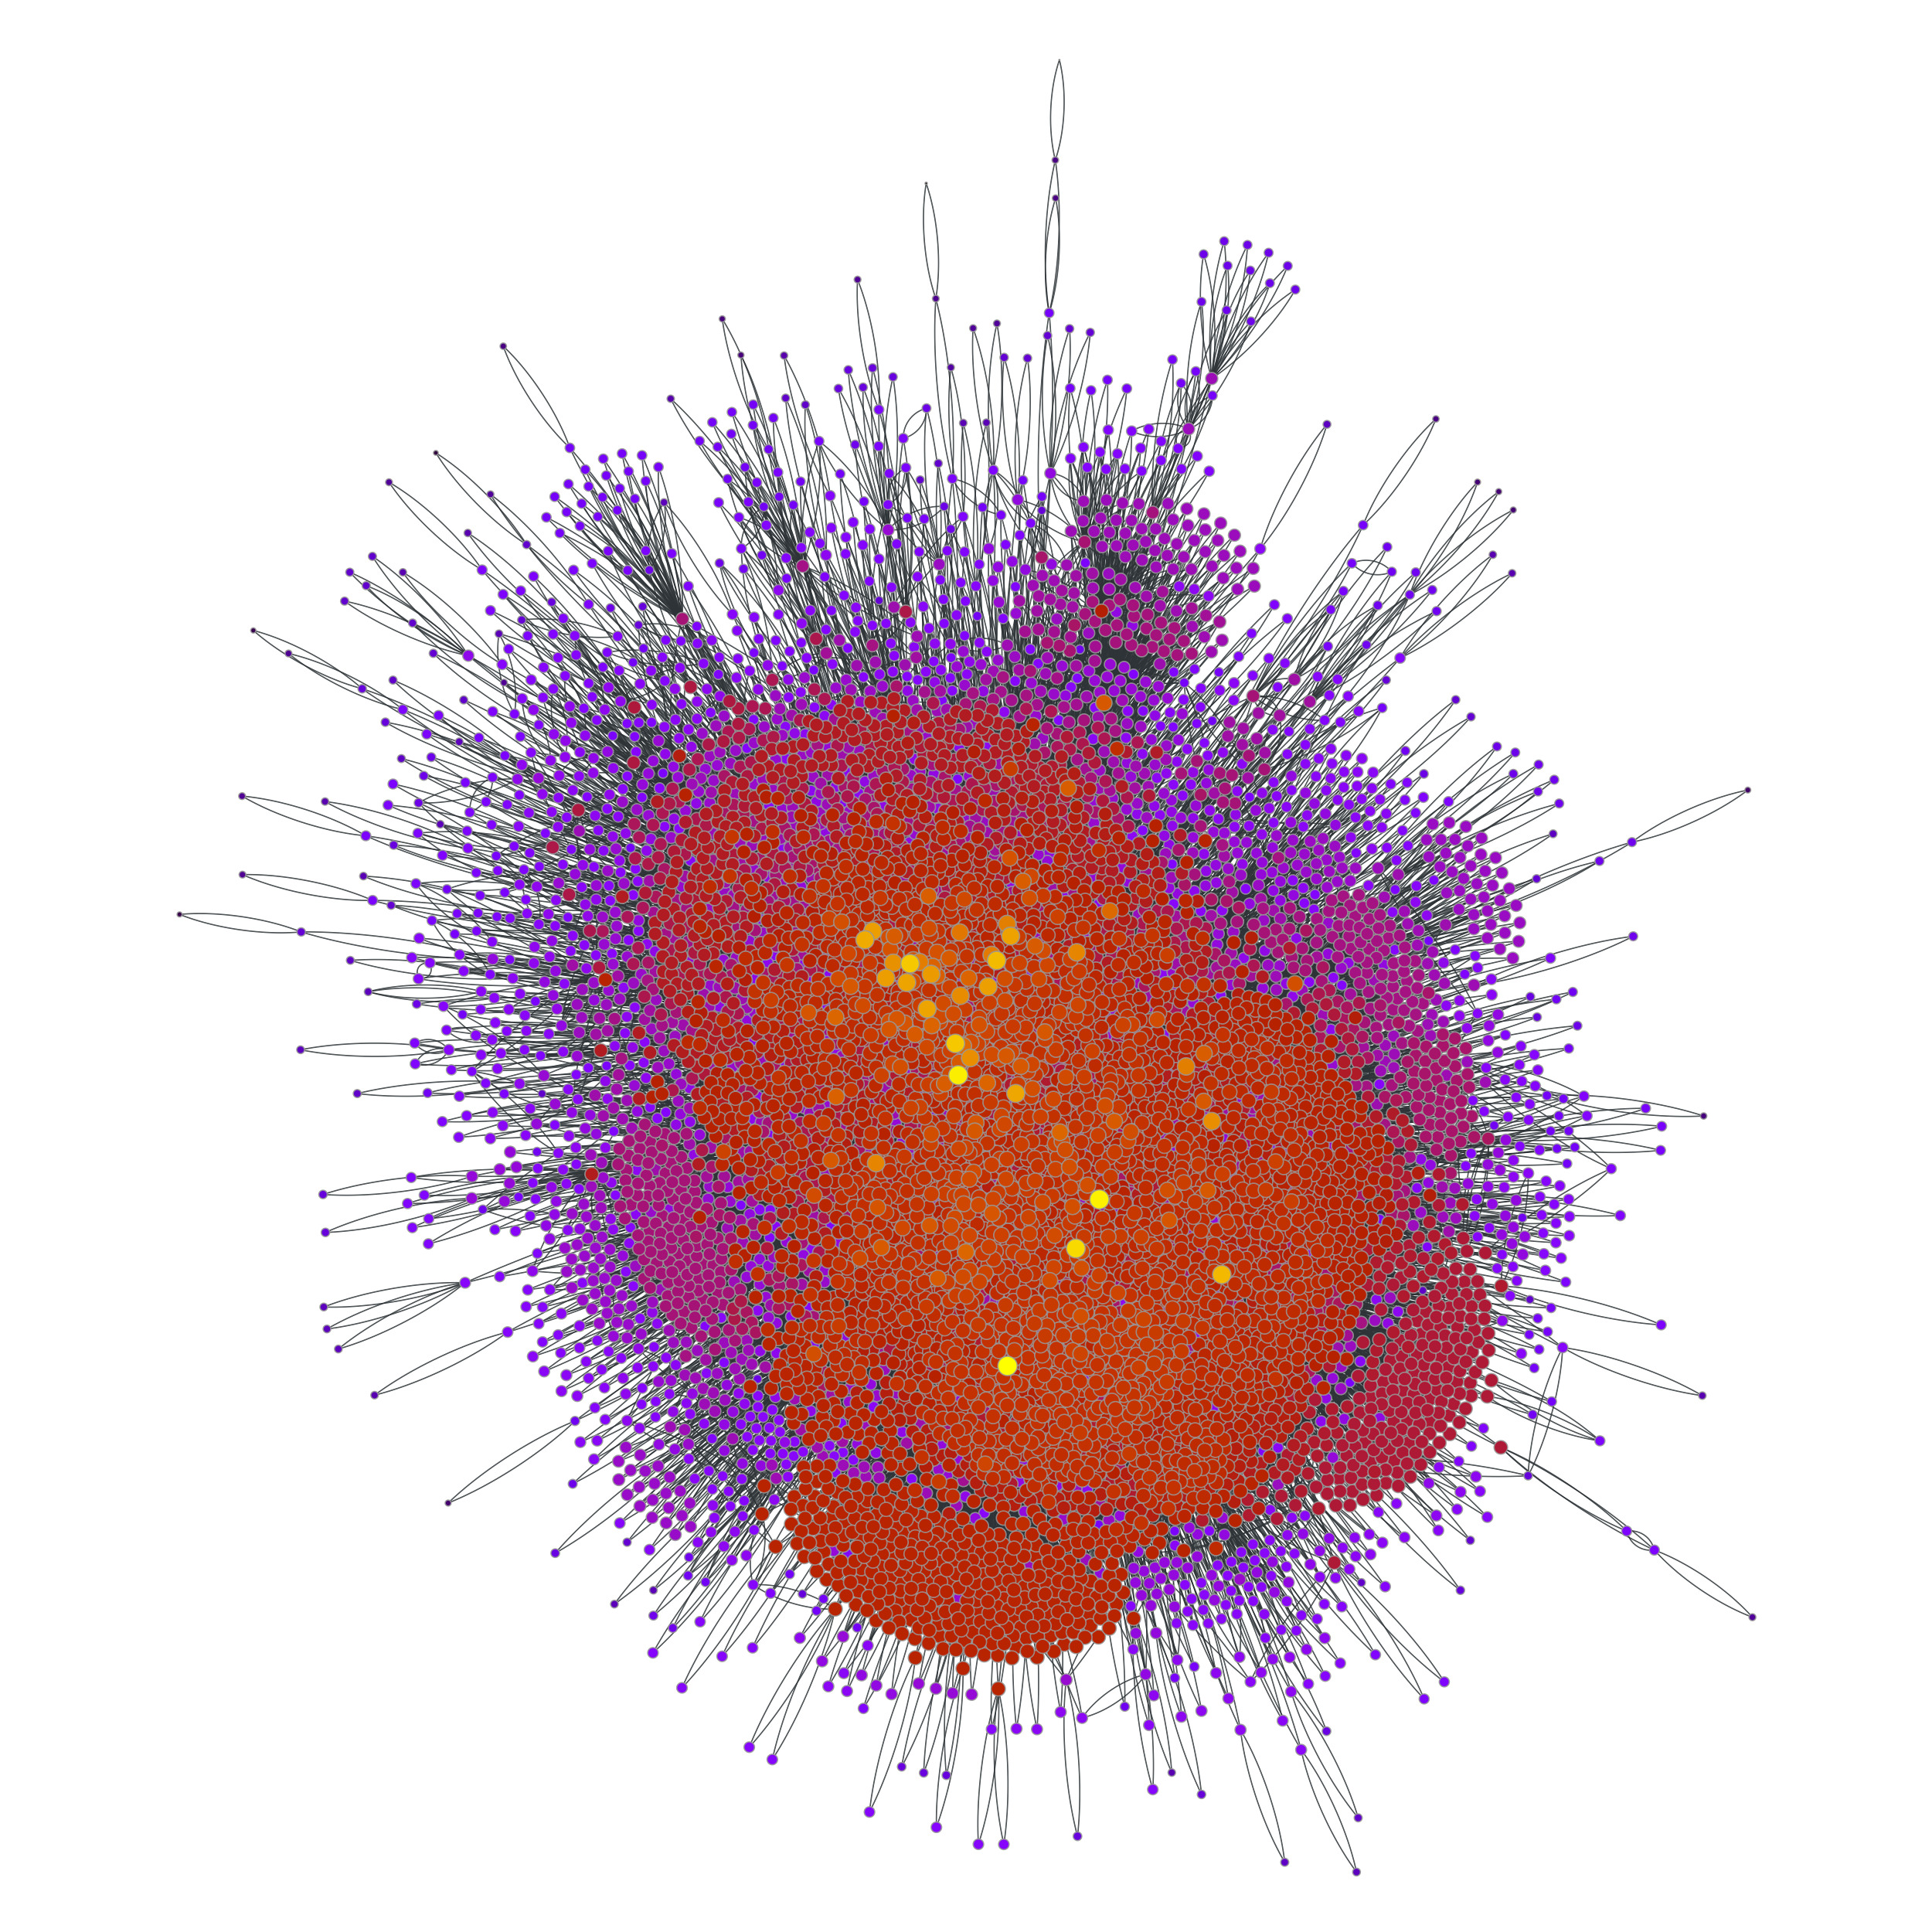
\includegraphics[width=\textwidth]{closeness_8k}
	\caption{Działanie Betweenness Centrality  na przykładowym grafie}
\end{figure}
\FloatBarrier\FloatBarrier
\subsubsection{Przykład}
\begin{figure}[h]
	\centering
	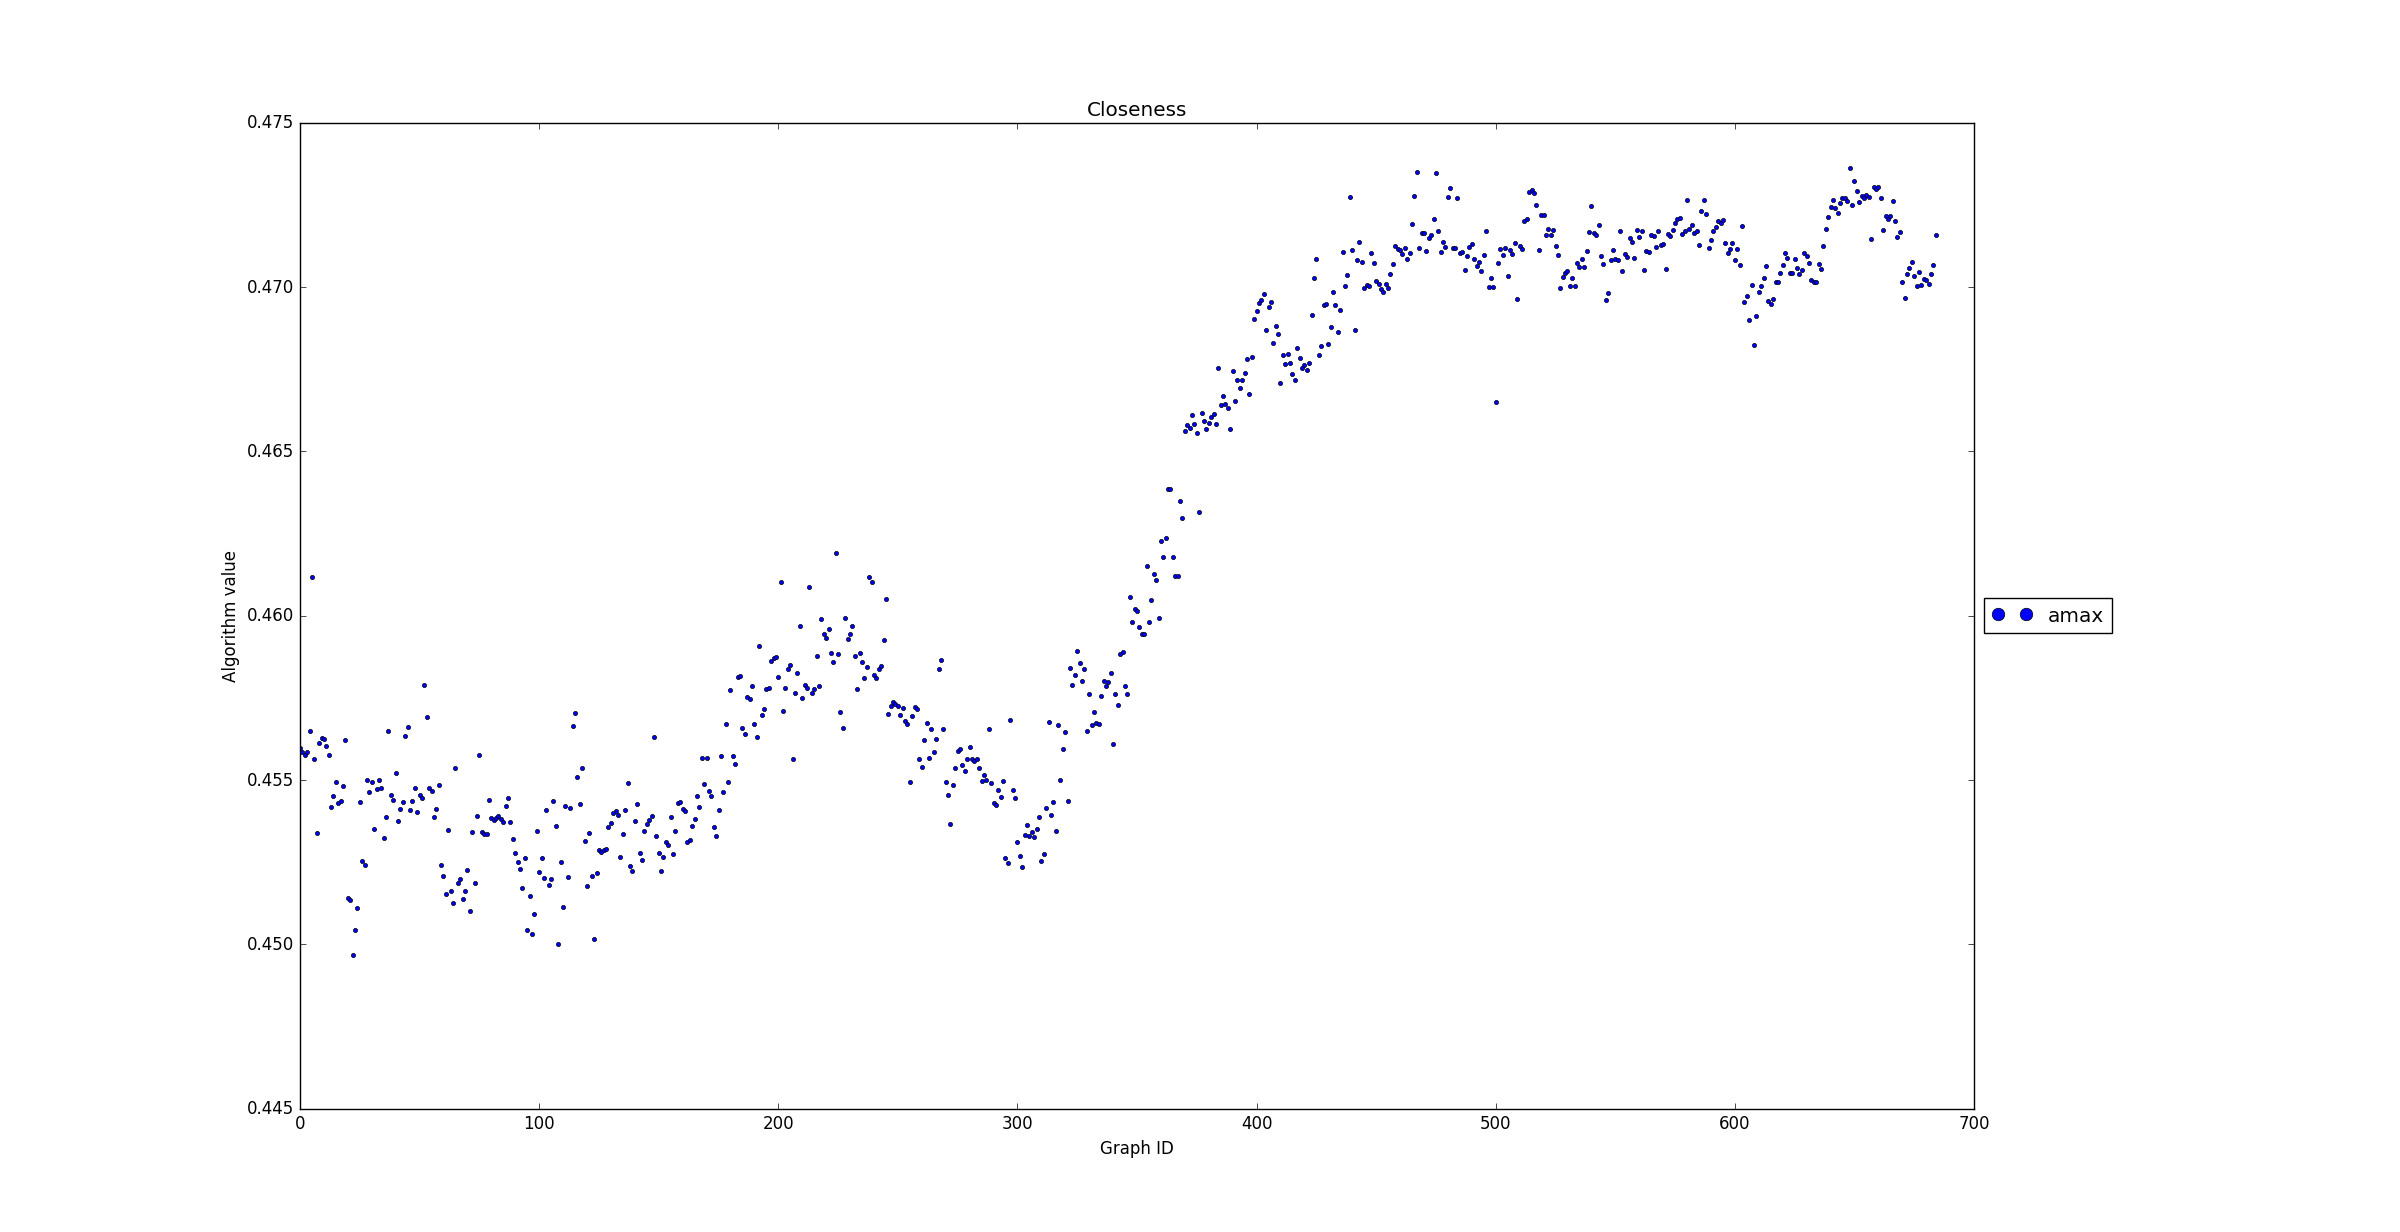
\includegraphics[width=\textwidth]{closeness_max}
	\caption{Działanie Betweenness Centrality  na przykładowym grafie}
\end{figure}
\FloatBarrier\FloatBarrier
\subsubsection{Przykład}
\begin{figure}[h]
	\centering
	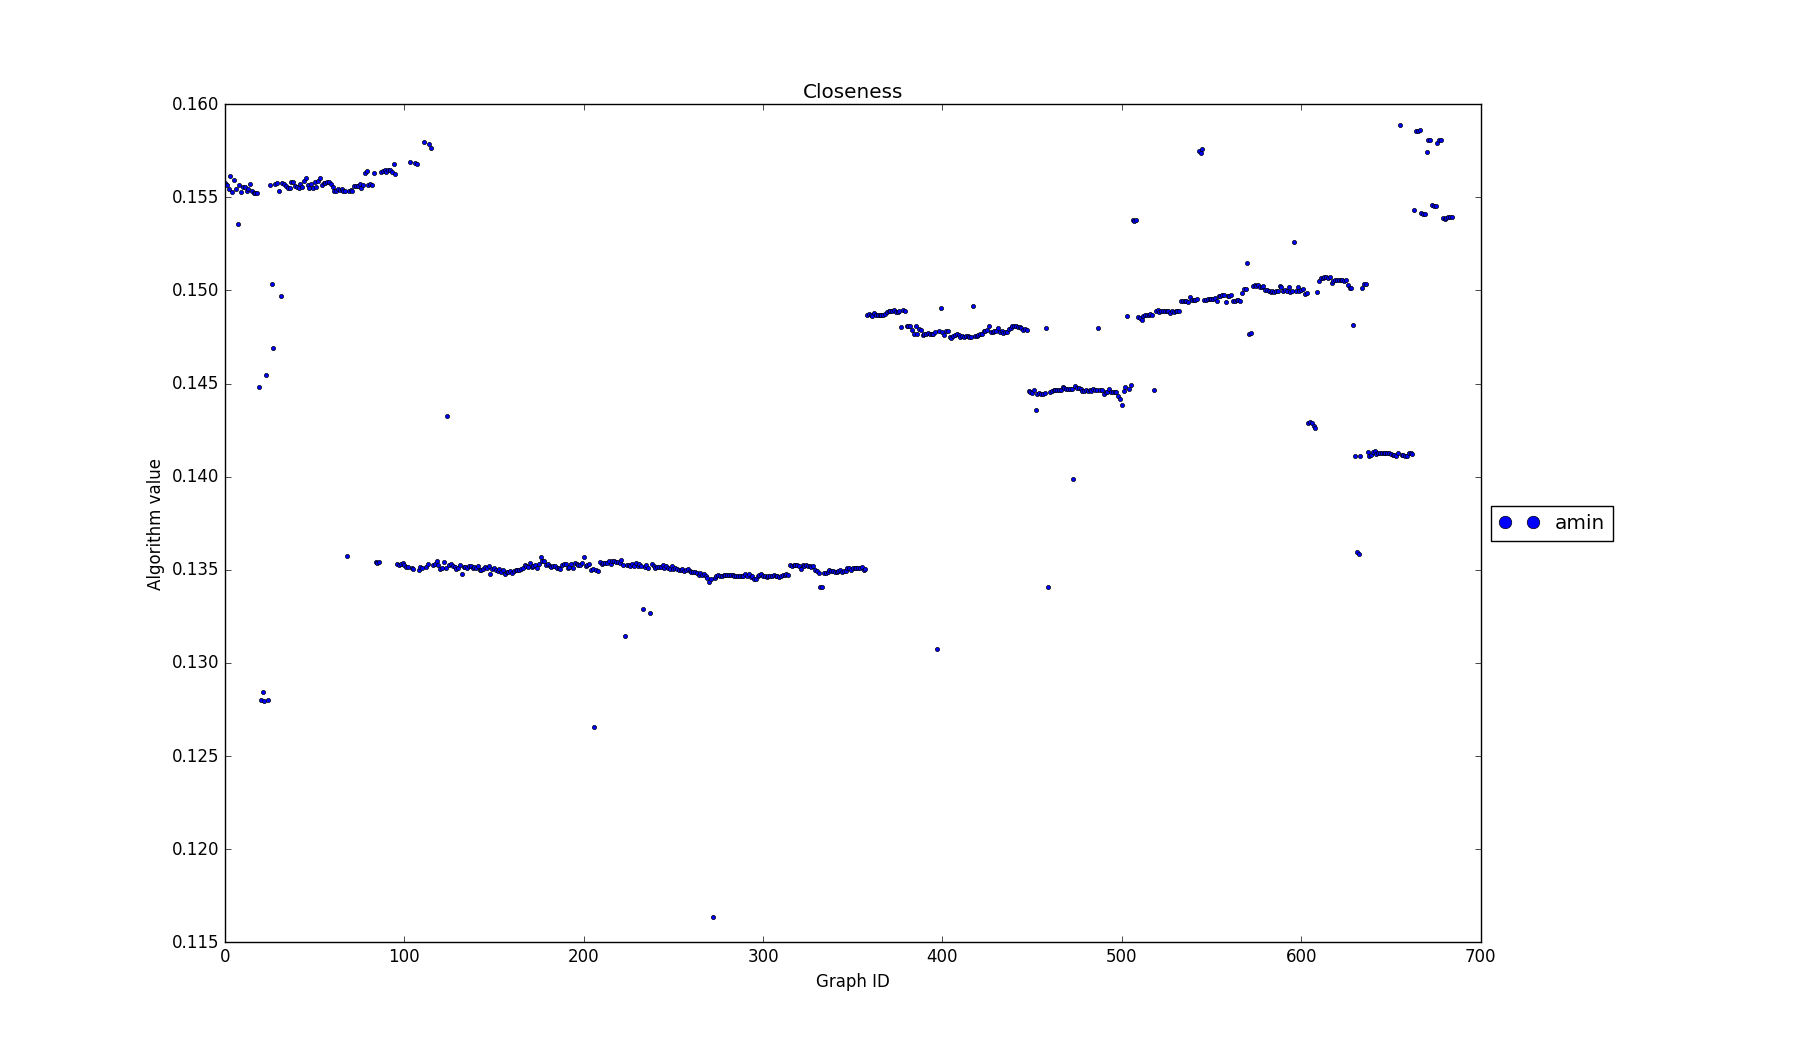
\includegraphics[width=\textwidth]{closeness_min}
	\caption{Działanie Betweenness Centrality  na przykładowym grafie}
\end{figure}
\FloatBarrier\FloatBarrier
\subsubsection{Przykład}
\begin{figure}[h]
	\centering
	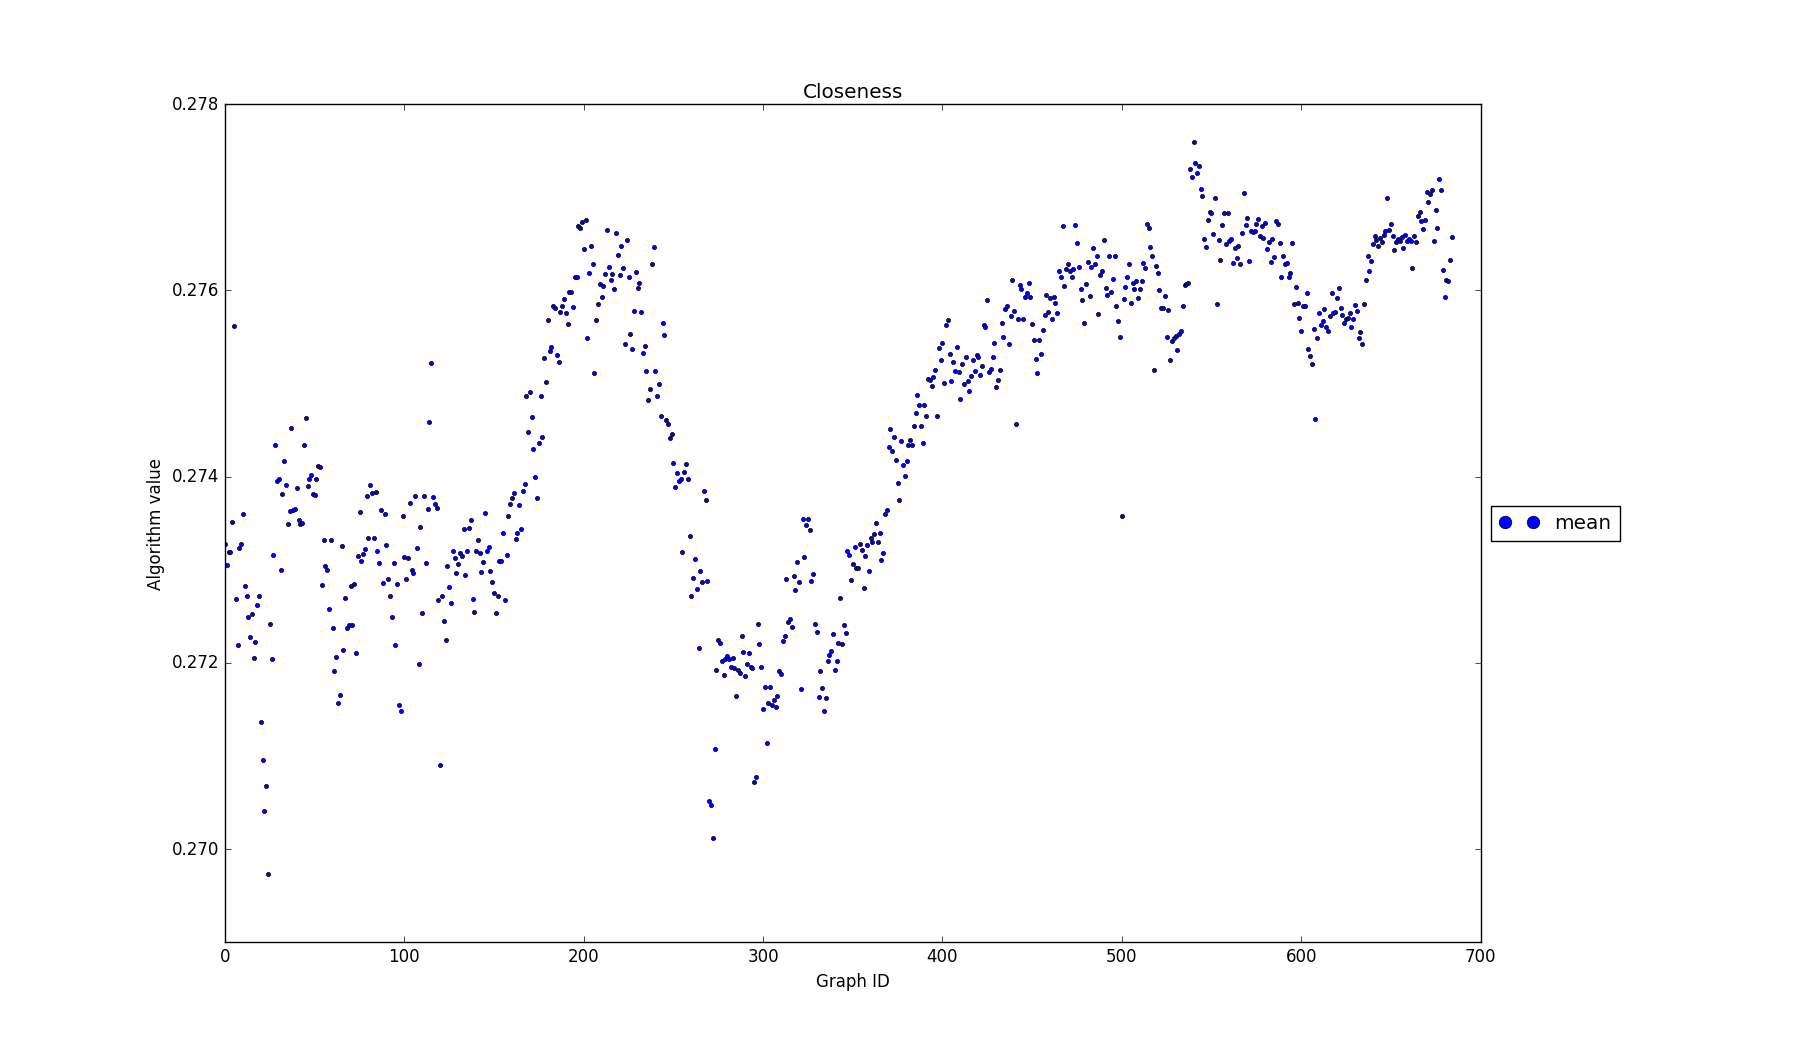
\includegraphics[width=\textwidth]{closeness_mean}
	\caption{Działanie Betweenness Centrality  na przykładowym grafie}
\end{figure}
\FloatBarrier\FloatBarrier
\subsubsection{Przykład}
\begin{figure}[h]
	\centering
	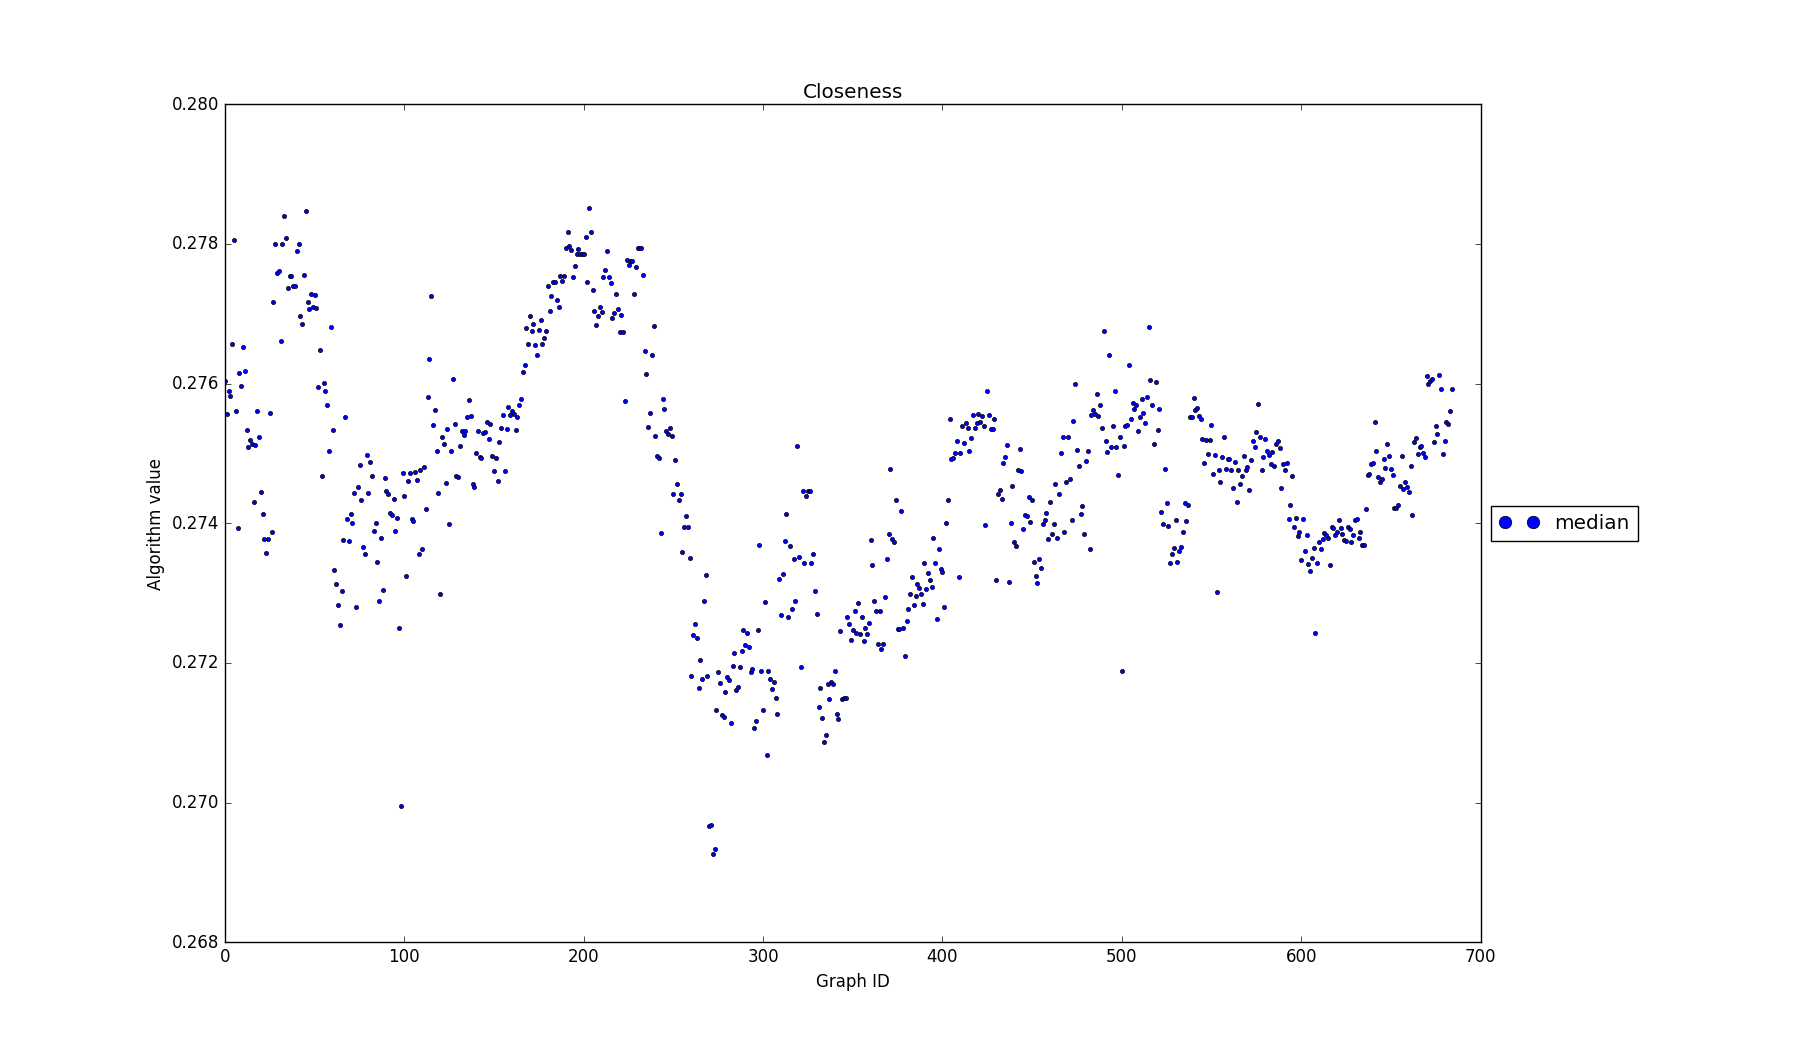
\includegraphics[width=\textwidth]{closeness_median}
	\caption{Działanie Betweenness Centrality  na przykładowym grafie}
\end{figure}
\FloatBarrier